\documentclass{article}
\usepackage{graphicx}
\usepackage[utf8]{inputenc}
\usepackage[T1]{fontenc}
\usepackage[portuguese]{babel}
\usepackage[authoryear]{natbib}
\usepackage{pgfgantt}
\usepackage{geometry}
\geometry{margin=2.5cm}

\title{Anteprojeto de Mestrado}
\author{Guilherme Mendes Rosa}
\date{Janeiro de 2026}

\begin{document}

\maketitle

\section{Introdução}

Atualmente, dois campos que despertam grande interesse tanto na academia quanto na indústria são a Robótica e a Inteligência Artificial. De acordo com \citet{Zamora2025Robotics}, essas áreas vêm ganhando destaque também no contexto da educação superior, refletindo seu crescente interesse e aplicação em diferentes domínios tecnológicos e acadêmicos. O avanço nessas áreas tem proporcionado impactos significativos na sociedade, permitindo a criação de soluções inovadoras que já fazem parte do cotidiano.

O projeto apresentado neste trabalho integra esses dois campos. Para isso, foi desenvolvido o robô LBot, cuja principal funcionalidade é a movimentação no espaço físico. A fim de possibilitar que esses movimentos sejam descritos de forma padronizada, foi criada uma linguagem de domínio específico (DSL), denominada \textit{LBot Movement Language} (LBML).

Entretanto, um desafio recorrente em aplicações de robótica é a necessidade de que o usuário aprenda comandos técnicos ou linguagens específicas para interagir com o robô. Essa exigência pode limitar a acessibilidade do sistema e dificultar sua adoção por usuários sem formação técnica. Diante desse cenário, este projeto parte da hipótese de que o uso de linguagem natural como meio de interação, aliado a modelos de aprendizado de máquina especializados, pode simplificar significativamente a comunicação entre humanos e robôs.

Neste contexto, o objetivo geral deste anteprojeto é investigar a tradução automática de comandos em português para a LBML, a partir de um conjunto de dados construído com base em interações reais e sintéticas. Como objetivos específicos, destacam-se: (i) o desenvolvimento de um simulador web que permita ao usuário comandar o robô por meio de linguagem natural; (ii) a constituição de um \textit{dataset} curado contendo comandos textuais e suas respectivas representações formais em LBML; (iii) a análise da eficácia de modelos baseados em arquiteturas do tipo Transformer na tarefa de tradução para linguagens de comando robótico; e (iv) a avaliação da qualidade das traduções, diferenciando erros sintáticos de erros semânticos.

A realização deste trabalho se justifica pela necessidade de tornar sistemas robóticos mais acessíveis e intuitivos. Além disso, propõe-se a criação de um modelo especializado e compacto, visando viabilizar sua operação em ambientes com recursos computacionais limitados (\textit{edge computing}) ou sem conexão constante à internet, dado que modelos de grande porte podem apresentar alta latência e custo computacional inviáveis nesses cenários \citep{Sun2019MobileBERT}.

\section{Referencial Teórico}

A interface entre linguagem natural e sistemas computacionais é um tema central na Robótica e na Inteligência Artificial, sendo o problema de \textit{Semantic Parsing} um de seus principais desafios. O \textit{Semantic Parsing} consiste na tradução de comandos em linguagem natural para representações formais e executáveis, como formas lógicas, consultas SQL ou código \citep{yu2018spider}.

No contexto deste trabalho, a utilização de uma linguagem de domínio específico, como a LBML, desempenha um papel fundamental ao restringir o vocabulário e a sintaxe aos comandos de movimentação do robô. Conforme discutido por \citet{Jimenez2017}, uma DSL concentra seu poder expressivo em um domínio particular e tende a empregar um conjunto restrito de notações e abstrações, o que simplifica o desenvolvimento e torna os comandos mais compreensíveis para os envolvidos. Essa restrição reduz ambiguidades da linguagem natural e contribui para a geração de comandos sintaticamente válidos.

Os avanços recentes em modelos baseados em arquiteturas Transformer têm demonstrado grande eficácia em tarefas de tradução automática \citep{Vaswani2017Attention}. O mecanismo de atenção presente nesses modelos permite capturar dependências complexas entre palavras e parâmetros, facilitando o alinhamento entre termos da linguagem natural e os elementos estruturais da LBML. Este trabalho investigará como tais arquiteturas se comportam quando treinadas em domínios restritos, em comparação a grandes modelos de linguagem generalistas.

Além disso, em aplicações robóticas, a confiabilidade da saída gerada é crítica. Torna-se necessário distinguir se um erro de tradução resulta em um comando inválido (erro de sintaxe) ou em um comando válido, porém incorreto em relação à intenção do usuário (erro semântico). Essa distinção é fundamental para avaliar a segurança e a robustez do sistema proposto.

\section{Metodologia}

A metodologia deste projeto está organizada em etapas incrementais. Inicialmente, será desenvolvido um simulador web que permita a interação do usuário com o robô por meio de uma interface de chat em linguagem natural.

Para a construção do conjunto de dados, será adotada uma abordagem híbrida. O usuário poderá expressar comandos livremente, os quais serão traduzidos preliminarmente para a LBML com o auxílio da API do ChatGPT. Os dados gerados sinteticamente passarão por uma etapa de validação e curadoria humana, a fim de evitar a propagação de erros e garantir a qualidade do treinamento.

Adicionalmente, o simulador permitirá a coleta de dados do tipo \textit{Gold Standard}, nos quais o usuário executará comandos manualmente na interface e descreverá, em linguagem natural, as ações realizadas. Essa estratégia visa capturar a variabilidade linguística real dos usuários.

Com base no conjunto de dados coletado e validado, será treinado um modelo de aprendizado de máquina baseado em arquiteturas Transformer, utilizando a biblioteca PyTorch. O objetivo é obter um modelo capaz de realizar a tradução de comandos em português para a LBML de forma autônoma.

A avaliação do modelo será realizada considerando dois níveis de sucesso. A métrica principal será a Taxa de Correspondência Exata (\textit{Exact Match Rate}), que quantifica a porcentagem de vezes em que o modelo gera exatamente o comando esperado. Complementarmente, será analisada a Taxa de Validade Sintática (\textit{Syntactic Validity Rate}), que mede a capacidade do modelo em gerar comandos estruturalmente válidos, ainda que semanticamente incorretos.

\section{Cronograma}

O cronograma do projeto está estruturado para um período total de 36 meses, contemplando tanto a fase como aluno especial quanto o período como aluno regular do curso de mestrado.
As atividades contemplam tanto a formação acadêmica quanto o desenvolvimento técnico e científico da pesquisa.

Nos primeiros 12 meses, período em que o discente atuou como aluno especial, foram cursadas três disciplinas. Paralelamente, iniciou-se o desenvolvimento do simulador do robô LBot, a definição da linguagem LBML e a realização de experimentos preliminares de tradução de comandos em linguagem natural, utilizando técnicas de \textit{prompt engineering} com modelos de linguagem.

O estado atual do simulador desenvolvido nesse período é apresentado na Figura~\ref{fig:estado-atual-simulador}.

\begin{figure}[h]
    \centering
    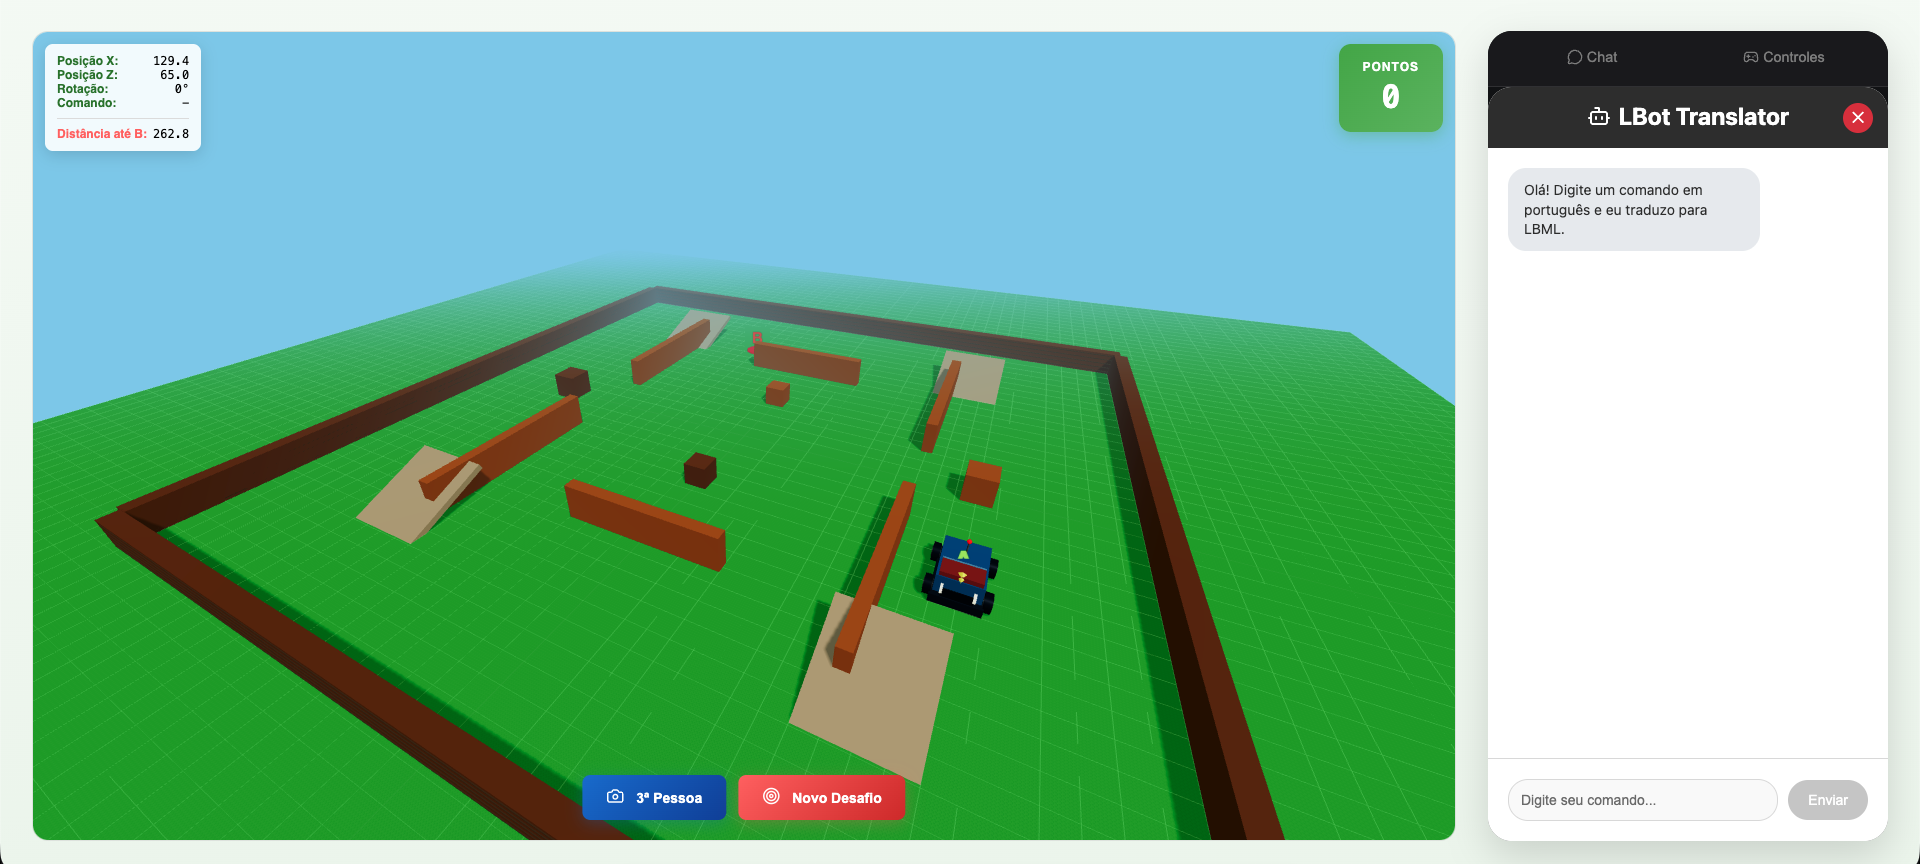
\includegraphics[width=0.95\linewidth]{simulador.png}
    \caption{Estado atual do simulador web do robô LBot.}
    \label{fig:estado-atual-simulador}
\end{figure}

Os 24 meses subsequentes correspondem ao período como aluno regular do programa. Nos primeiros 12 meses dessa etapa, estão previstas a conclusão das disciplinas restantes, a finalização do simulador, a coleta e curadoria do conjunto de dados e o treinamento inicial do modelo. Nos últimos 12 meses, o foco será o refinamento e a compactação do modelo, a realização das avaliações quantitativas e a finalização da redação da dissertação.

Ressalta-se que ajustes no cronograma poderão ocorrer em função dos resultados obtidos ao longo do desenvolvimento da pesquisa.

\subsection{Gráfico de Cronograma}

Para fins de leitura do gráfico, considera-se que o mês 1 corresponde a março de 2025 e o mês 36 corresponde a fevereiro de 2028. Dessa forma, as disciplinas iniciam sempre em março.

\begin{center}
\begin{ganttchart}[
    hgrid,
    vgrid,
    x unit=0.22cm,
    y unit chart=0.6cm,
    bar height=0.6,
    title height=1
]{1}{36}

\gantttitle{Aluno especial}{12}
\gantttitle{Ano 1}{12}
\gantttitle{Ano 2}{12} \\

\ganttbar{Disciplinas (aluno especial)}{3}{12} \\
\ganttbar{Desenvolvimento inicial do simulador e LBML}{3}{12} \\
\ganttbar{Experimentos preliminares com LLMs}{6}{12} \\

\ganttbar{Disciplinas (aluno regular)}{15}{24} \\
\ganttbar{Estágio de docência}{13}{16} \\
\ganttbar{Finalização do simulador web}{13}{18} \\
\ganttbar{Coleta e curadoria do dataset}{17}{22} \\
\ganttbar{Treinamento inicial do modelo}{21}{24} \\
\ganttbar{Exame de Inglês}{20}{20} \\
\ganttbar{Seminário (SIC)}{18}{21} \\

\ganttbar{Redação da dissertação}{13}{36} \\
\ganttbar{Refinamento e compactação do modelo}{25}{30} \\
\ganttbar{Avaliação quantitativa}{29}{33} \\
\ganttbar{Qualificação}{29}{29} \\
\ganttbar{Defesa}{35}{36} \\

\end{ganttchart}
\end{center}

\bibliographystyle{plainnat}
\bibliography{references}

\end{document}